\documentclass[11pt,a4paper]{article}
\usepackage[utf8]{inputenc}
\usepackage{amsmath,amsfonts,amssymb}
\usepackage{graphicx}
\usepackage{geometry}
\geometry{margin=1in}
\usepackage{booktabs}
\usepackage{hyperref}
\usepackage{float}

\title{\textbf{EE3621: Digital Signal Processing} \\ \Large Lecture 2: LTI Systems, Convolution, Stability \& Difference Equations \\ \large (III B.Tech EEE)}
\author{Lecture Notes (40-Minute Plan)}
\date{}

\usepackage{xcolor}
\definecolor{darkbg}{HTML}{0d121f}
\definecolor{lighttext}{HTML}{e2e8f0}
\definecolor{primary}{HTML}{8b5cf6}
\definecolor{secondary}{HTML}{0dd5c5}

\pagecolor{darkbg}
\color{lighttext}

\hypersetup{
    colorlinks=true,
    linkcolor=secondary,
    urlcolor=secondary
}

\begin{document}

\maketitle

\section{Lecture Plan \& Objectives (40 Minutes Breakdown)}
\begin{itemize}
    \item \textbf{00:00 -- 05:00 (5 mins):} Review of System Properties \& Introduction to LTI Systems.
    \item \textbf{05:00 -- 15:00 (10 mins):} Derivation of the Convolution Sum \& Graphical Steps.
    \item \textbf{15:00 -- 22:00 (7 mins):} Properties of Discrete-Time Convolution (with proofs).
    \item \textbf{22:00 -- 30:00 (8 mins):} LTI Causality, BIBO Stability (with proof), and Step Response.
    \item \textbf{30:00 -- 38:00 (8 mins):} Constant-Coefficient Difference Equations: Homogeneous \& Particular Solutions.
    \item \textbf{38:00 -- 40:00 (2 mins):} Checkpoints \& Quick Q\&A.
\end{itemize}

\noindent\rule{\textwidth}{0.5pt}

\section{Derivation of the Convolution Sum}
An LTI system is completely characterized by its impulse response $h[n] = \mathcal{T}\{\delta[n]\}$.
By the sifting property, any input $x[n]$ is expressed as:
\begin{equation}
x[n] = \sum_{k=-\infty}^{\infty} x[k] \delta[n-k]
\end{equation}
Applying linearity and time-invariance of $\mathcal{T}$:
\begin{equation}
y[n] = \mathcal{T}\{x[n]\} = \sum_{k=-\infty}^{\infty} x[k] \mathcal{T}\{\delta[n-k]\} = \sum_{k=-\infty}^{\infty} x[k] h[n-k]
\end{equation}
This is the convolution sum, denoted as $y[n] = x[n] * h[n]$ (see Figure~\ref{fig:conv_steps}).

\begin{figure}[H]
\centering
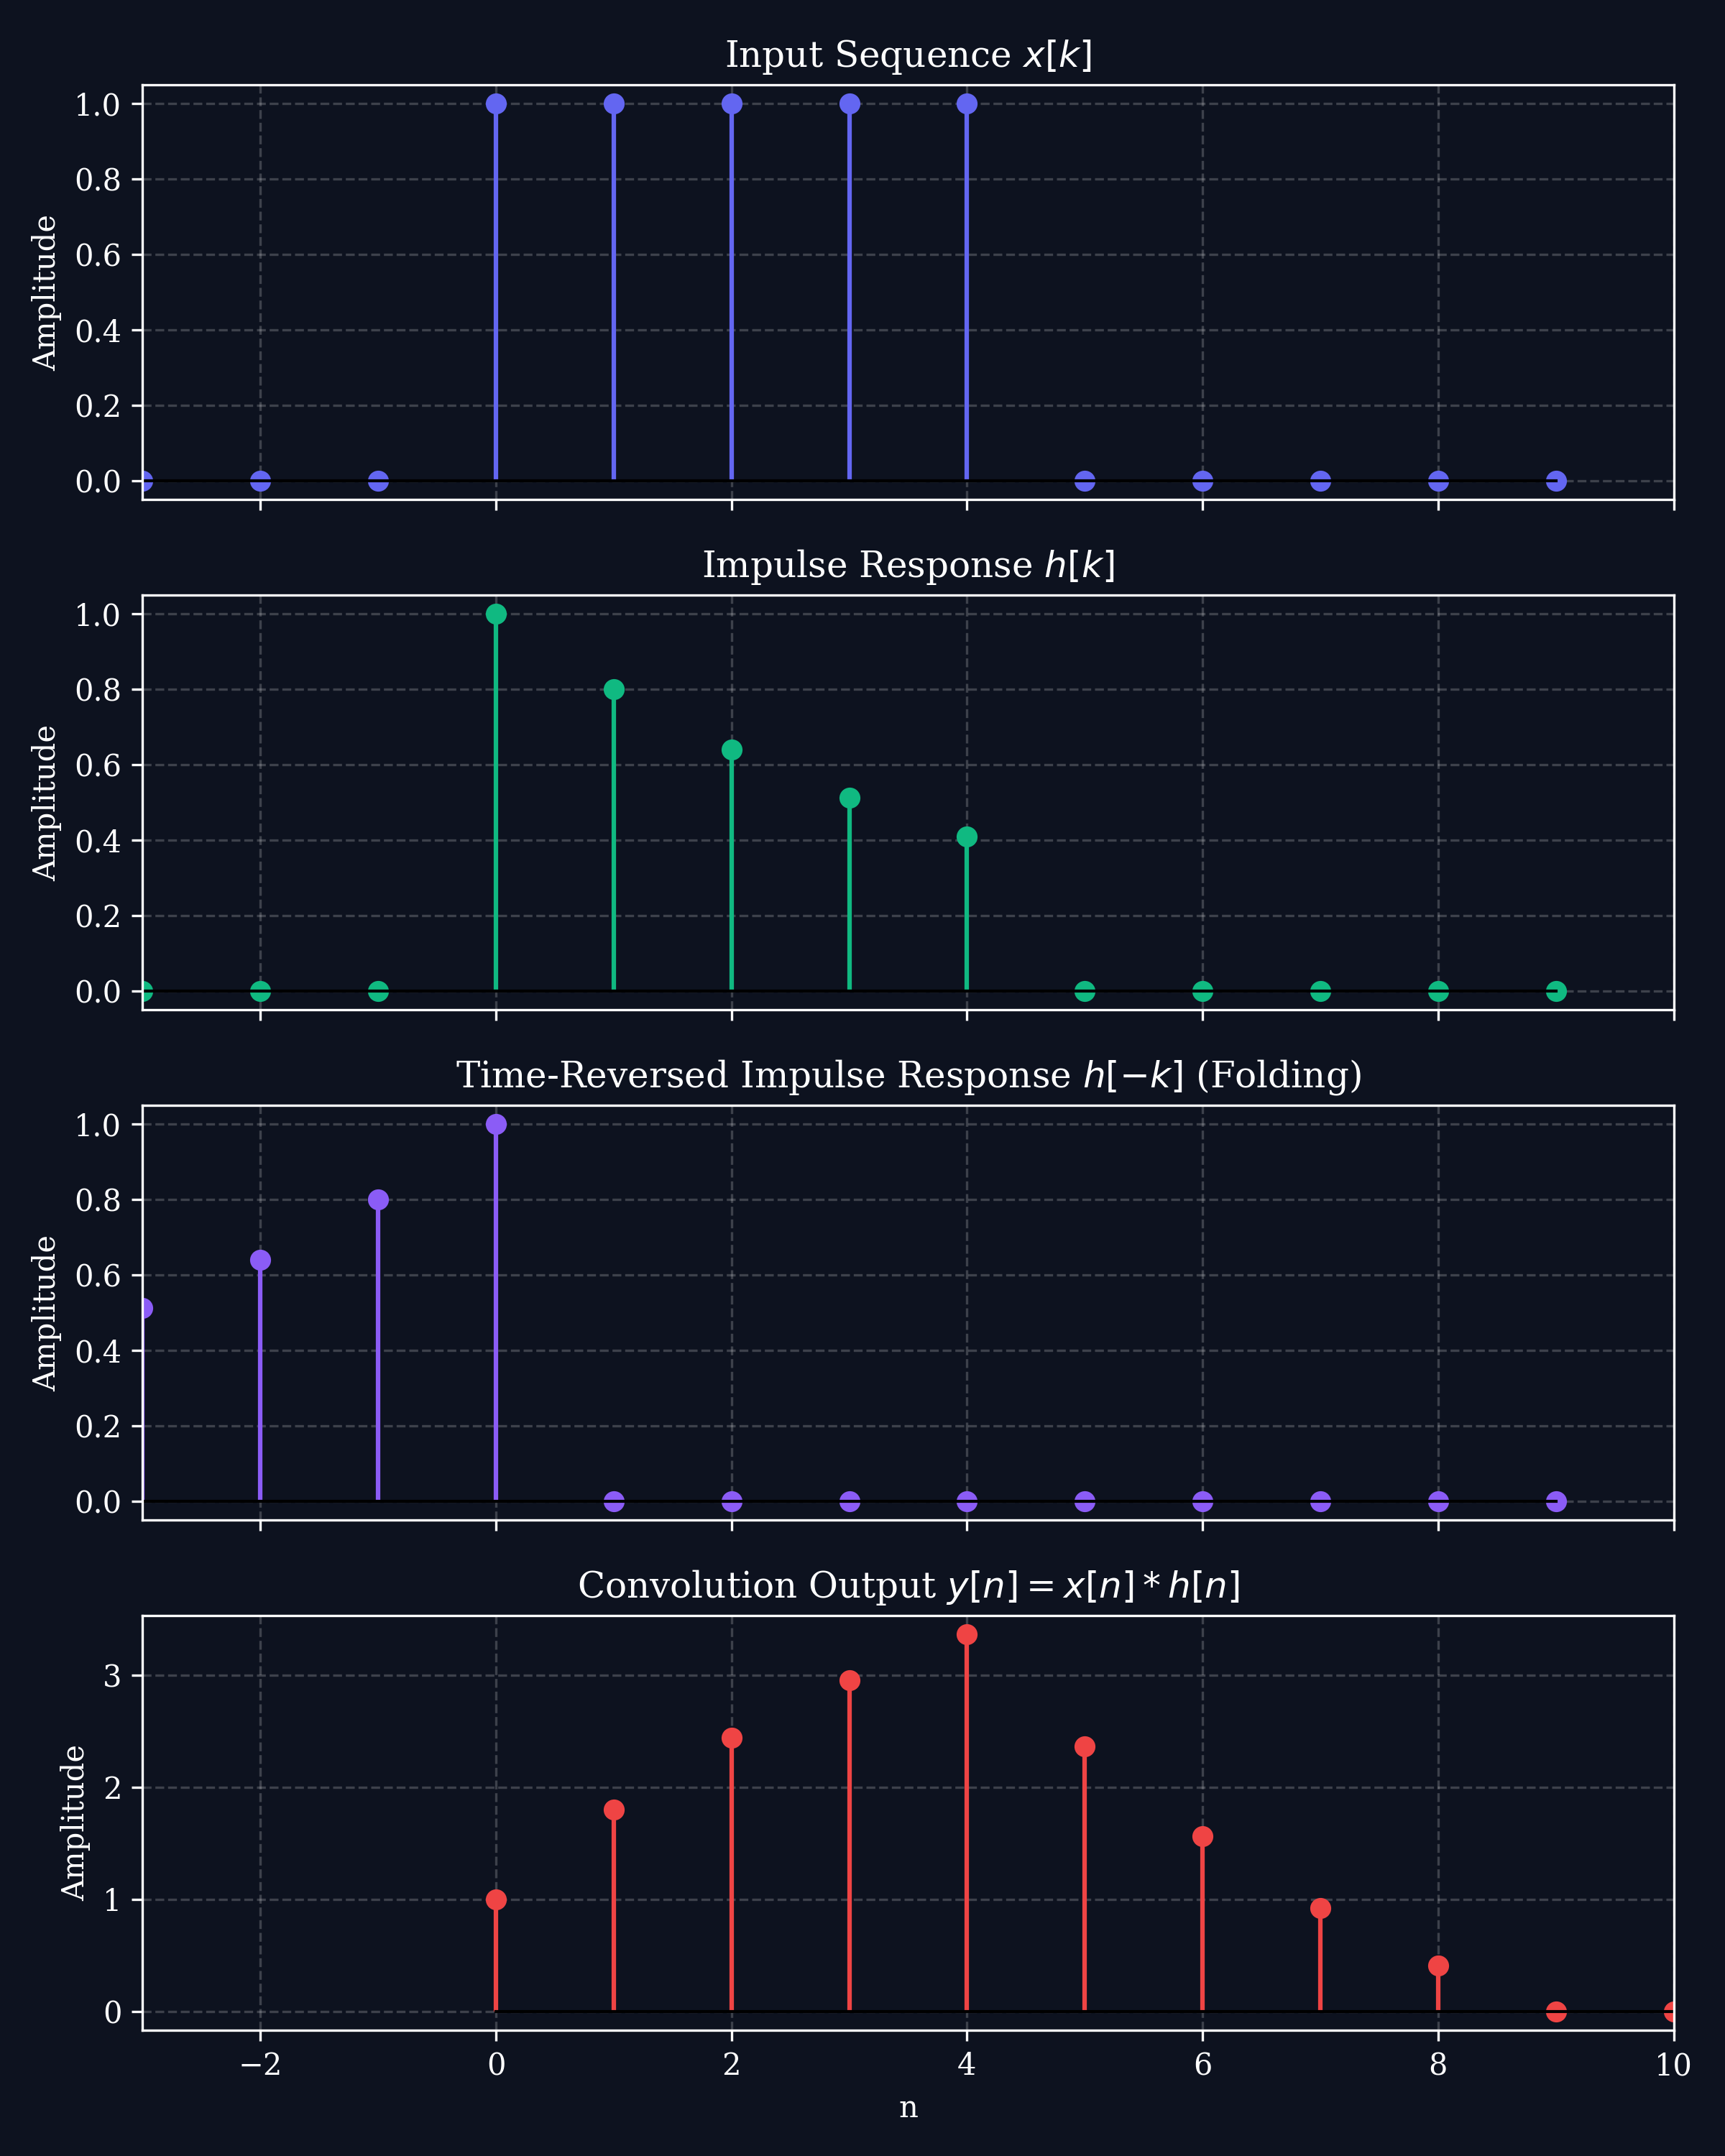
\includegraphics[width=0.85\textwidth]{images/convolution_steps.png}
\caption{Step-by-step graphical progression of convolution: folding, shifting, multiplication, and summation.}
\label{fig:conv_steps}
\end{figure}

\section{Properties of Discrete-Time Convolution}
\subsection{Commutativity}
\begin{equation}
x[n] * h[n] = h[n] * x[n]
\end{equation}
\textit{Proof:} Let $m = n-k \Rightarrow k = n-m$.
\begin{equation}
x[n] * h[n] = \sum_{k=-\infty}^{\infty} x[k]h[n-k] = \sum_{m=-\infty}^{\infty} x[n-m]h[m] = h[n]*x[n]
\end{equation}

\subsection{Associativity and Distributivity}
\begin{align}
(x[n] * h_1[n]) * h_2[n] &= x[n] * (h_1[n] * h_2[n]) \\
x[n] * (h_1[n] + h_2[n]) &= x[n] * h_1[n] + x[n] * h_2[n]
\end{align}

\subsection{Shifting Property}
If $y[n] = x[n] * h[n]$, then:
\begin{equation}
x[n-n_1] * h[n-n_2] = y[n - n_1 - n_2]
\end{equation}

\section{Causality, BIBO Stability \& Step Response}
\subsection{Causality}
An LTI system is causal if and only if:
\begin{equation}
h[n] = 0 \quad \forall n < 0
\end{equation}

\subsection{BIBO Stability}
An LTI system is BIBO stable if and only if its impulse response is absolutely summable:
\begin{equation}
S = \sum_{n=-\infty}^{\infty} |h[n]| < \infty
\end{equation}
\textit{Proof:} If $|x[n]| \le M_x$, then:
\begin{equation}
|y[n]| \le \sum_{k=-\infty}^{\infty} |x[k]| |h[n-k]| \le M_x \sum_{m=-\infty}^{\infty} |h[m]| = M_x S < \infty
\end{equation}
Stability profiles are shown in Figure~\ref{fig:lti_stability}.

\begin{figure}[H]
\centering
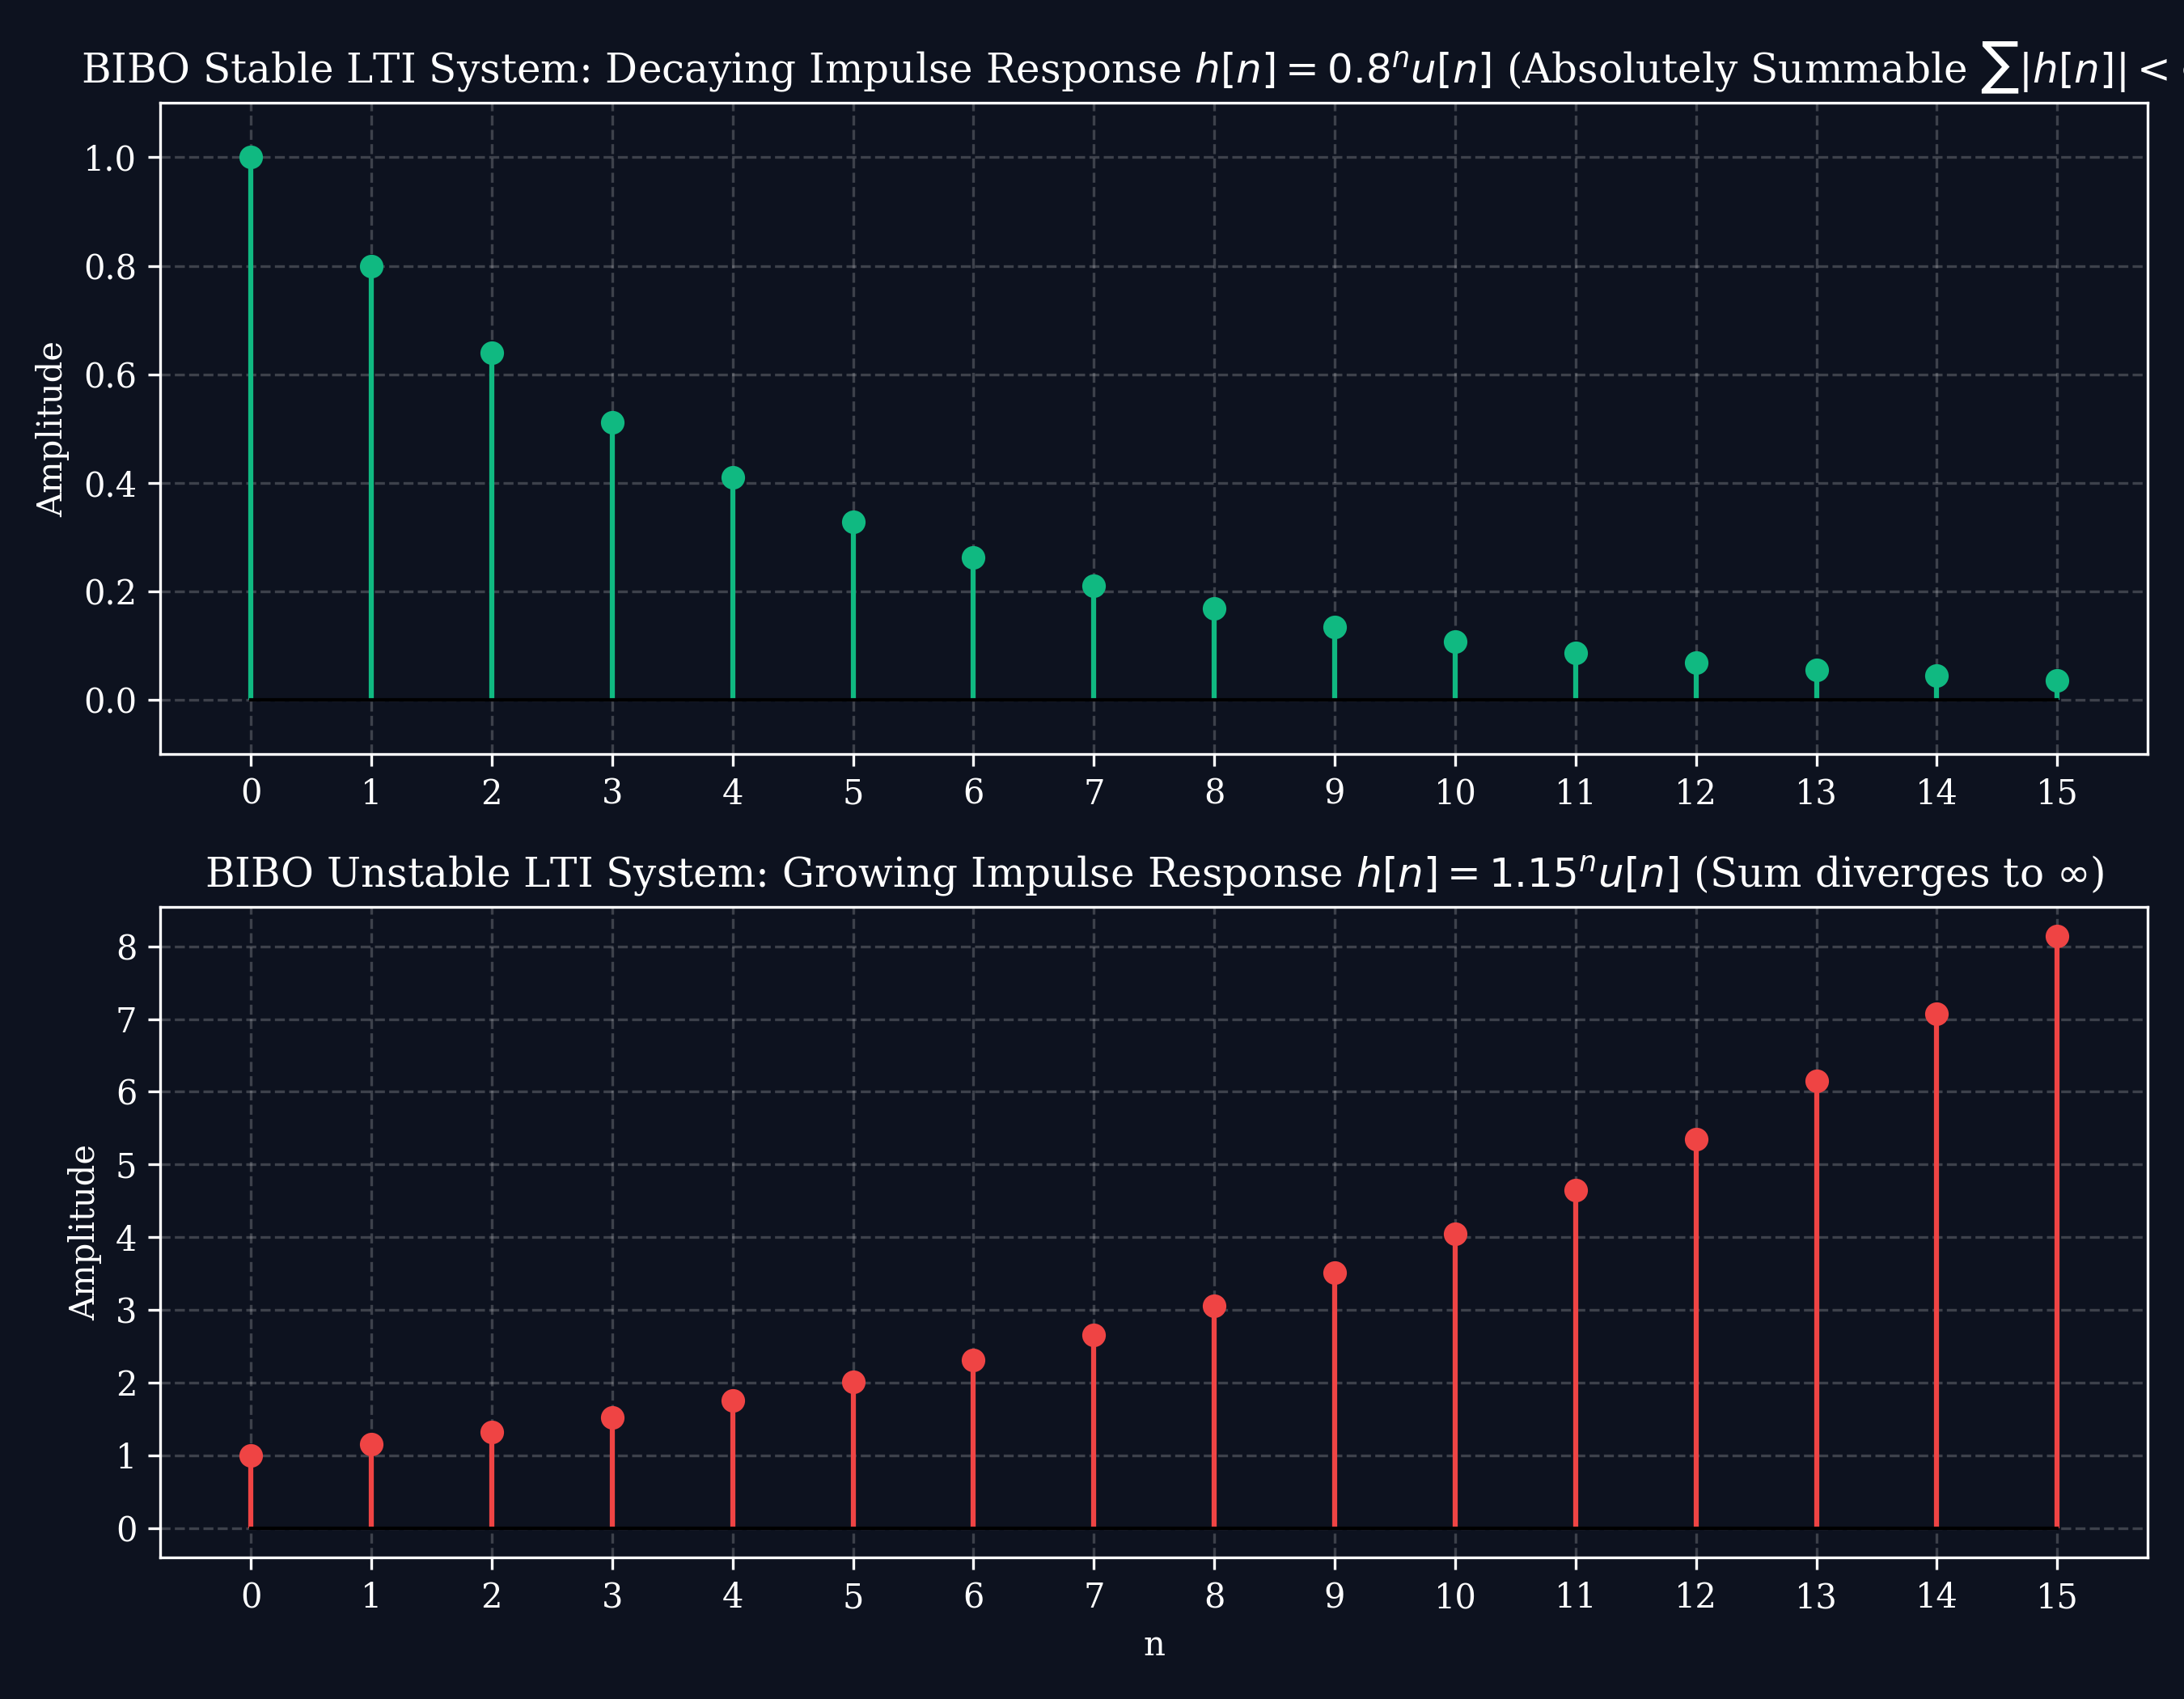
\includegraphics[width=0.85\textwidth]{images/lti_stability.png}
\caption{Impulse response profiles for stable and unstable discrete systems.}
\label{fig:lti_stability}
\end{figure}

\subsection{Step Response}
The unit step response is defined as:
\begin{equation}
s[n] = h[n] * u[n] = \sum_{k=-\infty}^{n} h[k]
\end{equation}
The impulse response is recovered by:
\begin{equation}
h[n] = s[n] - s[n-1]
\end{equation}

\section{Analytical Convolution Example (Infinite Sequences)}
Let $x[n] = a^n u[n]$ ($0 < a < 1$) and $h[n] = u[n]$.
\begin{equation}
y[n] = \sum_{k=-\infty}^{\infty} a^k u[k] u[n-k]
\end{equation}
For $u[k]u[n-k] \ne 0$, we require $0 \le k \le n$.
\begin{itemize}
    \item For $n < 0$: $y[n] = 0$.
    \item For $n \ge 0$:
    \begin{equation}
    y[n] = \sum_{k=0}^{n} a^k = \frac{1 - a^{n+1}}{1 - a}
    \end{equation}
\end{itemize}
Thus: $y[n] = \left(\frac{1 - a^{n+1}}{1 - a}\right) u[n]$.

\section{Constant-Coefficient Difference Equations}
Discrete-time LTI recursive systems are described by difference equations:
\begin{equation}
y[n] + \sum_{k=1}^{N} a_k y[n-k] = \sum_{k=0}^{M} b_k x[n-k]
\end{equation}
The total solution is $y[n] = y_h[n] + y_p[n]$.

\subsection{Homogeneous Solution $y_h[n]$}
Set $x[n] = 0$, yielding:
\begin{equation}
y_h[n] = C \lambda^n \quad \Longrightarrow \quad \lambda^N + a_1\lambda^{N-1} + \dots + a_N = 0
\end{equation}
For distinct roots $\lambda_k$, the homogeneous solution is:
\begin{equation}
y_h[n] = \sum_{k=1}^{N} C_k \lambda_k^n
\end{equation}

\subsection{Particular Solution $y_p[n]$}
Represented by trial functions corresponding to the inputs, e.g., $y_p[n] = K_p$ for constant inputs, or $y_p[n] = K_p \beta^n$ for exponential inputs $x[n] = A \beta^n$.

\end{document}
